%!TEX root = thesis.tex

\chapter{Evaluation}
\label{chapter:evaluation}

In this chapter, we describe the evaluation of the tool built. The evaluation is performed by using two separate methods: we evaluate the efficiency of development process with the software effort and complexity metrics presented in chapter \ref{chapter:methods}, and visualization effectiveness with guidelines by \citet{kraak_cartographic_1998} complemented by visualization heuristics by \citet{zuk_heuristics_2006} and map objectives by \citet{schlichtmann_visualization_2002} presented in chapter \ref{section:visualizationprinciples}. As using either of the methods requires a baseline project, we decided to implement a number of sister projects as defined by \citet{kitchenham_evaluating_1998}. In this chapter, the visualizations built during sister projects are referred to with the term ``reference visualization'' while the visualizations built with Thematic.js are referred to with ``Thematic.js visualization''. \fixme{Are these terms clear enough?}

\section{Defining the Evaluated Cases}

The visualization tool should be able to visualize a large variety of data. Moreover, the benefits of reusable software are typically emphasized when examining a large number of relatively similar cases \citep{frakes_software_1996}. However, in order to keep the scope of this work manageable, we decided to evaluate a set of visualization cases listed below.

\paragraph{Alko stores in Finland}
Store locations are most naturally visualized using a dot map. Alko provides an unsupported representational state transfer (REST) API\footnote{\url{http://www.alko.fi/api/store/mapmarkers?language=fi}} for fetching data of Alko stores. The data is in a non-standard ``flat dot'' format (see appendix \ref{appendix:flatdotformat}). Therefore, we decided to visualize Alko store locations using a dot map. The map should display all Alko stores in an effective fashion, with clustering support for markers in order to avoid map cluttering. This case is later referred to as ``store map''.

\paragraph{Earthquakes in California}
Earthquakes have two fundamental data axes: location and magnitude. Therefore, earthquakes are best visualized using a proportional symbol map with the size of the symbol representing magnitude. United States Geological Survey provides historical earthquake data\footnote{\url{http://earthquake.usgs.gov/earthquakes/search/}}, and we decided to visualize earthquakes in California since January 1, 1900. The data is available in a Comma-Separated Values (CSV) format which is can be trivially transformed to ``flat dot'' JSON format. This case is later referred to as ``earthquake map''.

\paragraph{Circulation of the Biggest Finnish Newspapers}
\fixme{Describe this}

\paragraph{Voter Turnout in Finnish Presidential Election of 2012}
The Finnish Ministry of Interior provides regional voter turnout data of the presidential election of 2012\footnote{\url{http://tulospalvelu.vaalit.fi/TP2012K2/s/aanaktiivisuus/aanestys1.htm}}. This data is provided in electoral district and municipality level. We decided to visualize the turnout in municipality level, using municipality data by the Finnish Land Survey\footnote{\url{http://www.maanmittauslaitos.fi/en/opendata}}. The municipality data is provided in GeoJSON format by Teemu Tiilikainen\footnote{\url{https://github.com/varmais/maakunnat}}. These data can be combined to create an effective choropleth visualization of regional turnout. The data should be normalized in quantized fashion, i.e., using thresholds to create a discrete color range. This case is later referred to as ``election map''.

\paragraph{Share of People with No Secondary Education in Finland}
Statistics Finland\footnote{\url{http://www.tilastokeskus.fi/}} provides provincial data on the education of the population of Finland in CSV format. This can be combined with province data by the Finnish Land Survey\footnote{\url{http://www.maanmittauslaitos.fi/en/opendata}} to create an effective choropleth visualization. The data should be normalized in linear fashion, i.e., using continuous color range. This case is later referred to as ``education map''.

\paragraph{Travel Times to a Single Destination}
Travel times to a destination can be visualized using an isarithmic map. We decided to visualize travel times to Futurice headquarters\footnote{\url{http://futurice.com/contact\#helsinki}} using public transport. The travel times can be obtained by using Travel Time Visualization Utility for HSL Reittiopas\footnote{\url{https://github.com/pyryk/reittiopas-travel-times}} which provides the data in an approximated ``flat dot'' format. The data should be normalized in a quantized fashion to emphasize isarithmic contours. This case is later referred to as ``simple travel times map''.

\paragraph{Travel Times to Multiple Destinations}
In addition to visualizing travel times to a single destination, we decided to evaluate a case for displaying travel times to multiple destinations. The travel times are obtained with the method defined in the previous paragraph, and combined using a weighted average method. Like in the previous case, the data should be normalized in a quantized fashion. This case is later referred to as ``complex travel times map''.

~

While the visualized data is arbitrarily selected, the cases are picked to reflect the typical usage of visualizations. Choropleth map and isarithmic map are the most frequenly used thematic mapping methods \citep[chap.~14-15]{slocum_thematic_2014} and therefore it is beneficial to the evaluation to examine multiple visualizations with those methods.

In order to better model typical real-life use cases, and to be usable on the web, the visualization cases include also a generic application structure and HTML features such as application caching and bookmarking support which are required for web applications.

\section{Implementing Sister Projects}

We implemented seven separate sister project visualizations with no visualization library to compare to visualization cases as defined in the previous section. The functionality of the visualizations was designed to reflect the functionality of the evaluated visualizations as accurately as possible. Sister visualizations were implemented using HTML, CSS and JavaScript to enable straightforward comparison to the evaluated visualization cases. While we did not use any visualization library for the sister projects, we deemed using a generic mapping library such as Leaflet.js appropriate, because typically, creating map visualizations is not feasible without using one. Moreover, also Thematic.js uses Leaflet.js as a mapping library.

In order to better reflect the actual situations involving building visualizations, the sister projects were implemented in \emph{ad hoc} fashion, meaning that the design or architecture of the applications were not planned extensively beforehand. Also, no reuse of any form between visualizations was planned. However, during implementation, some design and code scavenging was done in order to speed up the development process. \fixme{The sister project code can be found in ...}

\section{Evaluating Efficiency of Development}

We evaluated the efficiency of development by several metrics: software code length (number of physical (LOC) and logical (LLOC) lines of code), cyclomatic complexity (CC), Halstead difficulty (HD) and Halstead effort (HE). For measurements, we used ESComplex\footnote{\url{https://github.com/philbooth/escomplex}} for analyzing JavaScript programs. \fixme{What about HTML and CSS? Any way to measure these? Or is the effort for these considered equal in sister projects?}

We began the evaluation by measuring the aforementioned metrics for the visualizations. It should be noted that for these measurements, we did not include code from Thematic.js or other third party libraries. The measurements are shown in table \ref{table:efficiencymetrics}.

~

\LTcapwidth=\textwidth
\begin{longtable}{|l|c|c|c|c|c|}
\hline
\textbf{Visualization} & \textbf{LOC} & \textbf{LLOC} & \textbf{CC} & \textbf{HD} & \textbf{HE} \\ 
\hline
Thematic.js store & 12 & 12 & 1 & 7.31 & 4600 \\
Reference store & 126 & 85 & 10 & 23.6 & 96500 \\
Thematic.js earthquake & 15 & 14 & 1 & 8.38 & 6280 \\
Reference earthquake & 79 & 121 & 10 & 23.5 & 87400 \\
Thematic.js election & 26 & 29 & 2 & 10.9 & 12800 \\
Reference election & 141 & 101 & 14 & 23.8 & 107000 \\
Thematic.js education & 17 & 17 & 1 & 10.2 & 10200 \\
Reference education & 129 & 87 & 10 & 27.8 & 109000 \\
Thematic.js travel times simple & 27 & 28 & 2 & 10.8 & 9840 \\
Reference travel times simple & 184 & 129 & 12 & 29.4 & 182000 \\
Thematic.js travel times complex & 30 & 30 & 2 & 11.6 & 13300 \\
Reference travel times complex & 193 & 144 & 12 & 34.5 & 255000 \\
\hline
\caption{Measurements for developed visualizations, including only visualization-specific code. \fixme{Complete the table with real data} \fixme{Add the last missing visualization}}
\label{table:efficiencymetrics}
\end{longtable}

According to the results, using Thematic.js yields significantly lower complexity, difficulty and effort values when compared to using no visualization library. This is likely a direct result of Thematic.js providing an extensive map-specific visualization functionality, allowing the visualizer to concentrate on the visualized data. In practice, this means that when creating map visualizations, it is significantly more effective to use a library such as Thematic.js than to write the visualization from the ground up, given that the visualizer possesses -- or is able to achieve -- a general knowledge of the library functionality.

\fixme{Go through all evaluation cases in detail here - describe results and discuss why the results are as they are.}

However, it is likely that the results do not describe the most typical real-life scenarios completely accurately. It can be assumed that typically, visualizers do not possess knowledge of Thematic.js functionality beforehand and therefore effort for each line of code is considerably higher than when building the visualization from the ground up. In the results, this is reflected in rather high values for relative difficulty for Thematic.js visualizations as seen in figure \ref{fig:evaluationchart}.

\fixme{Qualitative analysis - don't repeat yourself etc.}

\begin{figure}[htbp]
  \begin{center}
    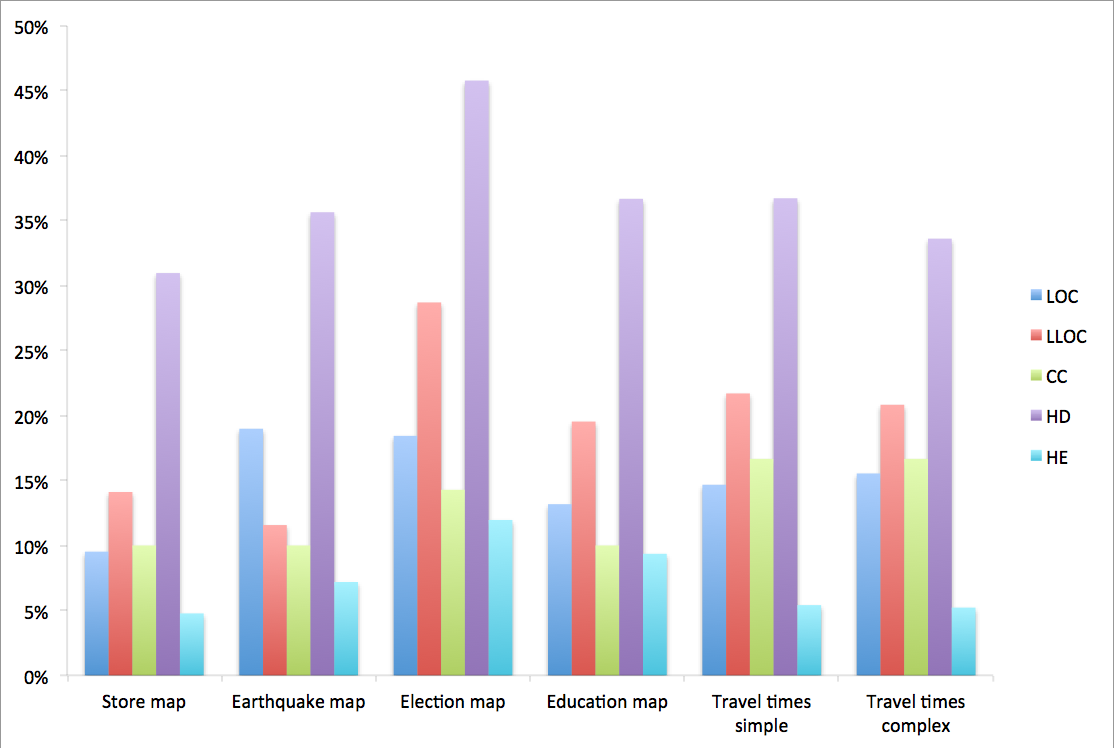
\includegraphics[width=\textwidth]{images/evaluation-results.png}
    \caption{Thematic.js visualization metrics for each case in relation to a corresponding reference visualization. \fixme{Is this the correct way of saying ``metric value in Thematic.js visualization / metric value in reference visualization''?} \fixme{Polish the chart}}
    \label{fig:evaluationchart}
  \end{center}
\end{figure}

Figure \ref{fig:evaluationchart} displays the ratio of Thematic.js visualization metrics for each visualization case to reference visualizations. The resulting metrics provide a good overview of the effort needed for Thematic.js visualizations compared to the using no visualization library.

Surprisingly, according to the results, using Thematic.js yields relatively high benefits for all metrics for the dot map visualization (store map). The reason for this may be that, even though dot map is an inherently simple visualization method, e.g., error handling and marker clustering support add complexity to the reference implementation. Moreover, as the Thematic.js visualization implementation for dot map visualization consists of only 12 lines of relatively simple code, the boilerplate code needed in the reference implementation causes the relative metrics to be notably low.

Relative metrics of proportional symbol (earthquake) map are approximately similar to the metrics of dot map. However, as the proportional symbol map is missing clustering support but involves symbol scaling functionality which is also needed in the Thematic.js implementation, the relative metrics are slightly more favorable to the reference implementation than in the dot map case. Nevertheless, also in proportional symbol case, using Thematic.js yields significant benefits compared to using no visualization framework, with Halstead effort measurement in Thematic.js implementation being under 10 \% of the corresponding measurement in the reference implementation.

\fixme{Add newspaper map}

Election map case yields the least benefits of all the evaluated cases, with Halstead difficulty being almost 50 \% and Halstead effort over 10 \% of the values for the reference implementation. This is likely due to the fact that the Leaflet.js mapping library provides a comprehensive GeoJSON polygon support used with choropleth visualizations. Therefore, the additional manual implementation needed for the reference case is relatively straightforward, the most effort needed being related to the coloring and showing values, the features that need to be implemented manually also in the Thematic.js implementation. That being said, even a simple choropleth map like this benefits considerably from the Thematic.js library.

In the education map case, using Thematic.js yields slightly greater benefits than in the election map. Like the election map, the education map uses choropleth mapping technique for visualization. However, the data in this case is already combined in GeoJSON format, so no manual combining is required. In both Thematic.js and reference implementations, an external coloring functionality is used, which reduces the size of the code bases. Especially the use of external coloring functionality reduces the Thematic.js relative complexity considerably, which leads to the more significant gains when using the library than in the election map case.

Both travel time maps yield highly similar results in measurements. This is likely due to the fact that both maps use isarithmic mapping method with relatively similar data, the only difference being the need for combining several data sources in the complex case. The data combining likely results in slightly lower values in Halstead difficulty and effort. However, in these cases, the Halstead effort metric is notably low, indicating that the effort for visualizing with Thematic.js taking only 5 \% of the effort of the reference implementation. This is probably due to the fact that even approximated isarithmic visualization requires a complex graphics implementation not supported directly by any mapping library.

Across all cases, the Thematic.js measurements indicate more significant differences in physical lines of code than logical lines of code. This is likely due to the fact that Thematic.js API is designed to encourage functional-style, chainable operations while traditional JavaScript APIs typically are imperative non-chainable. This is demonstrated in listing \ref{listing:chainableapi}. The chainable version can be used without line breaks, resulting in only 1 physical line of code, while with the API format in second example, it is not customary to combine the lines using only source code line. However, in practice, this has little effect on the actual effort needed as the underlying functionality stays largely similar.

\begin{lstlisting}[caption=Thematic.js API format. The code has been simplified to increase readability.,language=JavaScript,label=listing:chainableapi]
// chainable API supported by Thematic.js
map.addModule('voting', new Choropleth('percentage')
        .setScale(scale)
        .setData(data));

// non-chainable API typical for traditional 
// JavaScript libraries
var module = new Choropleth('percentage');
module.setScale(scale);
module.setData(data);
map.addModule('voting', module);
\end{lstlisting}

Additionally, in all the cases, Halstead difficulty measurements in Thematic.js implementations are 30 to 50 \% of the reference implementations while corresponding Halstead effort measurements are 4 to 12 \% of the reference implementations. This reflects the fact that the reference implementations consist largely of straightforward but laborious boilerplate code such as initializing the map. Thematic.js implementations consist mostly of data-specific initialization of the visualization, which is typically less straightforward but considerably more concise.

Lastly, it should be noted that while the measurements are suitable for comparing different cases, as absolute metrics they are approximate at best. In practice, this means that it is not sensible to assume that using Thematic.js reduces the effort needed to 10 \% of the original. However, in light of these results, it seems extremely likely that using the library for visualizations similar to the evaluated cases yields considerable benefits over building the visualizations from the ground up. For more details about the measurements, see appendix \ref{appendix:escomplex}.

\fixme{Should we try the evaluation with library code as part of Thematic.js numbers? If yes, add this here. If not, discuss this in discussion.}

\section{Evaluating Effectiveness of Visualizations}

In order to allow as reliable effort comparison as possible, we decided to implement the same functionality to reference visualizations as in Thematic.js visualizations. In practice, this results in the reference visualization being as similar feature-wise and visually to the Thematic.js visualization as possible. Therefore, it is not reasonable to compare the effectiveness of the corresponding reference and Thematic.js visualizations. Instead, we decided to evaluate the Thematic.js visualizations qualitatively, concentrating on how the library encourages the visualizer to create effective visualizations.

\subsection{Visualization Heuristics}

\citet{zuk_heuristics_2006} provide a list of heuristics for data visualizations. These heuristics are described in more detail in section \ref{section:visualizationprinciples}. We decided to use the heuristics as a basis for evaluating the created visualizations and Thematic.js functionality. We evaluated Thematic.js using a three-step scale: positive if the system has a positive effect (encourages creating effective visualizations) when compared to using no visualization library, neutral if the system has no effect, and negative if the system encourages creating ineffective visualizations. The full evaluation results can be seen in table \ref{table:heuristicsevaluation}.

% \begin{table}
\begin{longtable}{|p{3cm}|p{2.2cm}|p{7.8cm}|}
\hline
\textbf{Heuristic} & \textbf{Evaluation} & \textbf{Reasoning} \\ 
\hline
Visual variable & Neutral & Of map visualizations, this concerns mostly choropleth maps. Thematic.js choropleth maps do not ensure minimum geographical size for areas. However, using the default line weight ensures a minimum screen size of several pixels. \\[0.5em] % Ensure visual variable has sufficient length \\
Color order & Neutral & Thematic.js choropleth, dasymetric and isarithmic maps are primarily based on coloring the map. Moreover, the visualizer is given the possibility of freely choosing the colors. This may lead to situations when the visualizer chooses the colors inappropriately for displaying order. However, this situation is not different from the alternative situation of the visualizer creating the visualization without using a visualization library. \\[0.5em] % Don't expect a reading order from color \\
Color size & Neutral & Thematic.js does not provide any color-adjusting mechanisms based on the size of the element. \\[0.5em] % Color perception varies with size of colored item
Local contrast & Neutral & Thematic.js does not provide any color-adjusting mechanisms based on contrast. \\[0.5em] % Local contrast affects color
Color blindness & Neutral & Thematic.js does not provide any advice regarding color blindness. \\[0.5em] % Consider people with color blindness
Preattentive benefits & Neutral & Thematic.js provides and enforces spacial positioning of the data. However, this is fundamental to any geovisualization, and therefore, cannot be considered a positive trait of the library. \\[0.5em] % Preattentive benefits increase with field of view
Size variation & Positive & Thematic.js provides size variation in proportional symbol mapping to encourage the visualizer to emphasize quantitative variation in data. \\[0.5em] % Quantitative assessment requires position or size variation
Graphic dimensionality & Negative & Thematic.js does not enforce preserving dimensionality of the data, and in some cases, such as when using a proportional symbol map, it encourages the visualizer to increase dimensionality by displaying scala values using proportional symbols. \\[0.5em] % Preserve data to graphic dimensionality
Most data & Positive & Thematic.js encourages the visualizer to maximize data shown by providing support for several different mapping methods suitable for different kind of data. \\[0.5em] % Put the most data in the least space
No extra ink & Positive & Thematic.js provides data aggregation functionality to combine the relevant data. \\[0.5em] % Remove the extraneous (ink)
Gestalt laws & Positive & Thematic.js provides functionality to support Gestalt laws of grouping, such as using different symbols and sizes for different data points. However, not all Gestalt laws are considered. \\[0.5em] % Consider Gestalt Laws
Levels of detail & Positive & Thematic.js provides clustering functionality of dots and symbols. While currently there is no support for levels of detail for other mapping methods, the library does not prevent implementing this in the future. \\[0.5em] % Provide multiple levels of detail
Integrate text & Positive & Thematic.js supports attaching popups with textual content to data points, such as markers or choropleth areas. \\[0.5em]
Overview first & Positive & Thematic.js supports overview-first approach in most of the mapping methods. Dot and proportional symbol maps support marker clustering and choropleth, isarithmic and dasymetric maps support zooming in to show the details. \\[0.5em] % Provide overview first
Zoom and filter & Neutral & Thematic.js supports zooming of the map. However, support for filtering data on view-level is not provided. \\[0.5em]
Details on demand & Positive & Thematic.js supports attaching popups to data points for displaying additional details. \\[0.5em]
Relate & & Consider relationships among items \\[0.5em]
Extract & & Allow extraction of data and its subsets \\[0.5em]
History & & Keep history of actions \\[0.5em]
Uncertainty & & Expose uncertainty \\[0.5em]
Relationships & & Concretize relationships \\[0.5em]
Domain Parameters & & Determination of domain parameters \\[0.5em]
Multivariate & & Provide multivariate explanation \\[0.5em]
Cause \& effect & & Formulate cause \& effect \\[0.5em]
Hypotheses & & Confirm Hypotheses \\[0.5em]
\hline
\caption{Evaluation of Thematic.js according to heuristics presented by \citet{zuk_heuristics_2006}.}
\label{table:heuristicsevaluation}
\end{longtable}
% \end{table}

\fixme{Move the table to appendices. Add overview here.}

\begin{itemize}
	\item Heuristics by \citet{zuk_heuristics_2006}
	\item Objectives by \citet{schlichtmann_visualization_2002}
	\item Guidelines in \citet{kraak_cartographic_1998} (how do i say what to whom and is it effective)
\end{itemize}

You have done your work, but that's\footnote{By the way, do \emph{not} use
shorthands like this in your text! It is not professional! Always write out all
the words: ``that is''.} not enough. 

You also need to evaluate how well your implementation works.  The
nature of the evaluation depends on your problem, your method, and
your implementation that are all described in the thesis before this
chapter.  If you have created a program for exact-text matching, then
you measure how long it takes for your implementation to search for
different patterns, and compare it against the implementation that was
used before.  If you have designed a process for managing software
projects, you perhaps interview people working with a waterfall-style
management process, have them adapt your management process, and
interview them again after they have worked with your process for some
time. See what's changed.

The important thing is that you can evaluate your success somehow.
Remember that you do not have to succeed in making something spectacular; a
total implementation failure may still give grounds for a very good master's
thesis---if you can analyze what went wrong and what should have been done.

 
